\documentclass[a4paper,12pt]{article}

\usepackage[utf8x]{inputenc}
\usepackage[T2A]{fontenc}
\usepackage[english, russian]{babel}

% Опционно, требует  apt-get install scalable-cyrfonts.*
% и удаления одной строчки в cyrtimes.sty
% Сточку не удалять!
% \usepackage{cyrtimes}

% Картнки и tikz
\usepackage{graphicx}
\usepackage{tikz}
\usetikzlibrary{snakes,arrows,shapes}


% Некоторая русификация.
\usepackage{misccorr}
\usepackage{indentfirst}
\renewcommand{\labelitemi}{\normalfont\bfseries{--}}

% Увы, поля придётся уменьшить из-за листингов.
\topmargin -1cm
\oddsidemargin -0.5cm
\evensidemargin -0.5cm
\textwidth 17cm
\textheight 24cm

\sloppy

% Оглавление в PDF
\usepackage[
bookmarks=true,
colorlinks=true, linkcolor=black, anchorcolor=black, citecolor=black, menucolor=black,filecolor=black, urlcolor=black,
unicode=true
]{hyperref}

% Для исходного кода в тексте
\newcommand{\Code}[1]{\texttt{#1}}

\usepackage{verbatim}
\usepackage{fancyvrb}
\fvset{frame=leftline, fontsize=\small, framerule=0.4mm, rulecolor=\color{darkgray}, commandchars=\\\{\}}
\renewcommand{\theFancyVerbLine}{\small\arabic{FancyVerbLine}}


\title{Отчёт по лабораторной работе \\ <<Система доменных имён>>}
\author{(Зиновьев Денис, ИУ7-32м)}

\begin{document}

\maketitle

\tableofcontents

\section{Настройка системы DNS}

\subsection{Топология сети}

Топология сети и использыемые IP-адреса показаны на рис.~\ref{fig:network}.

\begin{figure}
\centering
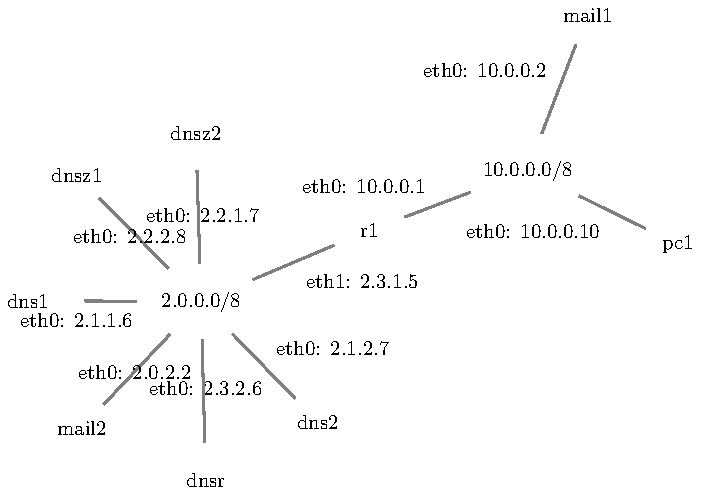
\includegraphics[width=\textwidth]{includes/network_gv.pdf}
\caption{Топология сети}
\label{fig:network}
\end{figure}

\subsection{Структура службы доменных имён}

Структура авторитетных серверов доменных имён показана на рис.~\ref{fig:dns}.

\begin{figure}
\centering
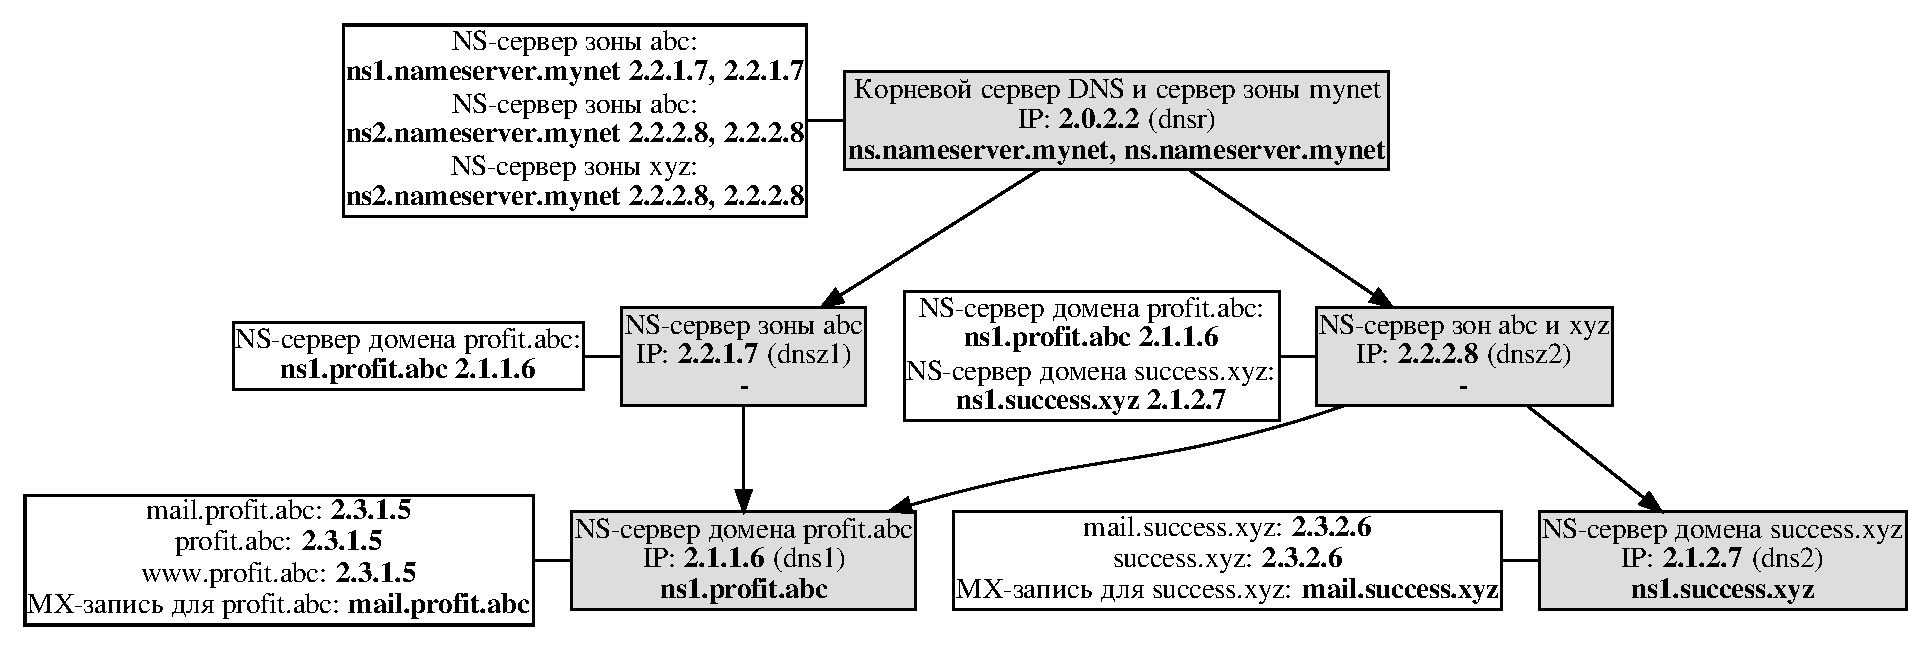
\includegraphics[width=\textwidth]{includes/dns_gv.pdf}
\caption{Структура службы доменных имён}
\label{fig:dns}
\end{figure}

\subsection{Прочие настройки}

Кеширующие DNS-серверы
\begin{itemize}
\item r1 (2.3.1.5);
\item mail2 (2.3.2.6);
\end{itemize}

Развёрнутые SMTP-серверы и используемые ими кеширующие DNS-серверы.
\begin{itemize}
\item mail1 использует кеширующий DNS (r1);
\item mail2 использует кеширующий DNS (mail2);
\end{itemize}


\section{Проверка настройки службы доменных имён}

\subsection{Проверка настройки записи типа MX для домена profix.abc}

\begin{verbatim}
mail2:~# dig @2.0.2.2 profit.abc MX
; <<>> DiG 9.5.0-P2 <<>> @2.0.2.2 profit.abc MX
; (1 server found)
;; global options:  printcmd
;; Got answer:
;; ->>HEADER<<- opcode: QUERY, status: NOERROR, id: 43361
;; flags: qr rd; QUERY: 1, ANSWER: 0, AUTHORITY: 2, ADDITIONAL: 2
;; WARNING: recursion requested but not available

;; QUESTION SECTION:
;profit.abc.			IN	MX

;; AUTHORITY SECTION:
abc.			86400	IN	NS	ns2.nameserver.mynet.
abc.			86400	IN	NS	ns1.nameserver.mynet.

;; ADDITIONAL SECTION:
ns1.nameserver.mynet.	86400	IN	A	2.2.1.7
ns2.nameserver.mynet.	86400	IN	A	2.2.2.8

;; Query time: 14 msec
;; SERVER: 2.0.2.2#53(2.0.2.2)
;; WHEN: Sat Dec 28 05:32:05 2019
;; MSG SIZE  rcvd: 112
\end{verbatim}

\begin{verbatim}
mail2:~# dig @2.2.1.7 profit.abc MX

; <<>> DiG 9.5.0-P2 <<>> @2.2.1.7 profit.abc MX
; (1 server found)
;; global options:  printcmd
;; Got answer:
;; ->>HEADER<<- opcode: QUERY, status: NOERROR, id: 25179
;; flags: qr rd; QUERY: 1, ANSWER: 0, AUTHORITY: 1, ADDITIONAL: 1
;; WARNING: recursion requested but not available

;; QUESTION SECTION:
;profit.abc.			IN	MX

;; AUTHORITY SECTION:
profit.abc.		86400	IN	NS	ns1.profit.abc.

;; ADDITIONAL SECTION:
ns1.profit.abc.		86400	IN	A	2.1.1.6

;; Query time: 1 msec
;; SERVER: 2.2.1.7#53(2.2.1.7)
;; WHEN: Sat Dec 28 05:41:00 2019
;; MSG SIZE  rcvd: 62
\end{verbatim}

\begin{verbatim}
mail2:~# dig @2.1.1.6 profit.abc MX

; <<>> DiG 9.5.0-P2 <<>> @2.1.1.6 profit.abc MX
; (1 server found)
;; global options:  printcmd
;; Got answer:
;; ->>HEADER<<- opcode: QUERY, status: NOERROR, id: 27466
;; flags: qr aa rd; QUERY: 1, ANSWER: 1, AUTHORITY: 1, ADDITIONAL: 2
;; WARNING: recursion requested but not available

;; QUESTION SECTION:
;profit.abc.			IN	MX

;; ANSWER SECTION:
profit.abc.		86400	IN	MX	10 mail.profit.abc.

;; AUTHORITY SECTION:
profit.abc.		86400	IN	NS	ns1.profit.abc.

;; ADDITIONAL SECTION:
mail.profit.abc.	86400	IN	A	2.3.1.5
ns1.profit.abc.		86400	IN	A	2.1.1.6

;; Query time: 5 msec
;; SERVER: 2.1.1.6#53(2.1.1.6)
;; WHEN: Sat Dec 28 05:43:42 2019
;; MSG SIZE  rcvd: 99
\end{verbatim}

Итоговая проверка: опрашиваем кеширующий DNS-сервер.

\begin{verbatim}
mail2:~# dig @127.0.0.1 profit.abc MX

; <<>> DiG 9.5.0-P2 <<>> @127.0.0.1 profit.abc MX
; (1 server found)
;; global options:  printcmd
;; Got answer:
;; ->>HEADER<<- opcode: QUERY, status: NOERROR, id: 6764
;; flags: qr rd ra; QUERY: 1, ANSWER: 1, AUTHORITY: 0, ADDITIONAL: 1

;; QUESTION SECTION:
;profit.abc.			IN	MX

;; ANSWER SECTION:
profit.abc.		86400	IN	MX	10 mail.profit.abc.

;; ADDITIONAL SECTION:
mail.profit.abc.	86400	IN	A	2.3.1.5

;; Query time: 9 msec
;; SERVER: 127.0.0.1#53(127.0.0.1)
;; WHEN: Sat Dec 28 05:48:31 2019
;; MSG SIZE  rcvd: 65
\end{verbatim}

\begin{verbatim}
mail2:~# ping profit.abc
PING profit.abc (2.3.1.5) 56(84) bytes of data.
64 bytes from 2.3.1.5: icmp_seq=1 ttl=64 time=10.2 ms
64 bytes from 2.3.1.5: icmp_seq=2 ttl=64 time=0.537 ms<Paste>
\end{verbatim}


\section{Проверка работы почтовой системы}

\subsection{Проверка MX-записи для домена profit.abc}

\begin{verbatim}
dns1:~# dig profit.abc MX

; <<>> DiG 9.5.0-P2 <<>> profit.abc MX
;; global options:  printcmd
;; Got answer:
;; ->>HEADER<<- opcode: QUERY, status: NOERROR, id: 35484
;; flags: qr aa rd; QUERY: 1, ANSWER: 1, AUTHORITY: 1, ADDITIONAL: 2
;; WARNING: recursion requested but not available

;; QUESTION SECTION:
;profit.abc.			IN	MX

;; ANSWER SECTION:
profit.abc.		86400	IN	MX	10 mail.profit.abc.

;; AUTHORITY SECTION:
profit.abc.		86400	IN	NS	ns1.profit.abc.

;; ADDITIONAL SECTION:
mail.profit.abc.	86400	IN	A	2.3.1.5
ns1.profit.abc.		86400	IN	A	2.1.1.6

;; Query time: 1 msec
;; SERVER: 127.0.0.1#53(127.0.0.1)
;; WHEN: Sat Dec 28 07:20:48 2019
;; MSG SIZE  rcvd: 99
\end{verbatim}

С узла dnsr отправили письмо на SMTP-сервер для адресата с адресом rootusr@success.xyz.

\begin{verbatim}
dns1:~# echo "some txt" | mail -s "subject1" root@profit.abc

dns1:~# tail -n 100 /var/log/exim4/mainlog
2019-12-28 07:18:25 1il6Mj-0000Kr-UU <= root@dns1 U=root P=local S=301
2019-12-28 07:18:26 1il6Mj-0000Kr-UU => root@profit.abc R=dnslookup T=remote_smtp H=mail.profit.abc [2.3.1.5]
2019-12-28 07:18:26 1il6Mj-0000Kr-UU Completed
\end{verbatim}

На машине с доменным именем mail.success.xyz появилось доставленное письмо.
\begin{verbatim}
From root@dns1 Sat Dec 28 07:18:26 2019
Return-path: <root@dns1>
Envelope-to: root@profit.abc
Delivery-date: Sat, 28 Dec 2019 07:18:26 +0000
Received: from [2.1.1.6] (helo=dns1)
by mail1 with esmtp (Exim 4.69)
(envelope-from <root@dns1>)
id 1il6Mk-0000Xi-0Y
for root@profit.abc; Sat, 28 Dec 2019 07:18:26 +0000
Received: from root by dns1 with local (Exim 4.69)
(envelope-from <root@dns1>)
id 1il6Mj-0000Kr-UU
for root@profit.abc; Sat, 28 Dec 2019 07:18:25 +0000
To: root@profit.abc
Subject: subject1
Message-Id: <E1il6Mj-0000Kr-UU@dns1>
From: root <root@dns1>
Date: Sat, 28 Dec 2019 07:18:25 +0000

some txt
\end{verbatim}

\end{document}
